\documentclass[final, usenames, dvipsnames]{beamer}
\mode<presentation>{\usetheme{GWU}}
\usepackage{poster_packages}

\DeclareSIUnit\year{yr}

\usepackage[orientation=landscape, width=121.92cm, height=91.44cm,scale=1.24,debug]{beamerposter} 
%\beamertemplategridbackground[0.1in] % grid for aligning stuff

%\setlength{\abovecaptionskip}{0.1cm}
%\setlength{\belowcaptionskip}{-0.3cm}

\def\newblock{} % Avoid the "\newblock undefined" error. See http://newsgroups.derkeiler.com/Archive/Comp/comp.text.tex/2008-07/msg00381.html"

%-----------------------------------------------------------
\newlength{\colsep}
\newlength{\onecolwidth}
\newlength{\twocolwidth}

\setlength{\paperwidth}{121.92cm} % 48in
\setlength{\paperheight}{91.44cm} % 36in


%\setlength{\onecolwidth}{0.23\textwidth} % Width of one column
%\setlength{\twocolwidth}{0.49\textwidth} % Width of two columns
\setlength{\onecolwidth}{28cm} % Width of one column
\setlength{\twocolwidth}{56cm} % Width of two columns
\newlength{\columnheight}
\setlength{\columnheight}{76.5cm}

\setbeamersize{text margin left=1.5cm,text margin right=0.5cm}

\listfiles

%-----------------------------
% MACROS
%-----------------------------
\def\Emph{\textcolor{RoyalBlue}}
%%%%%%%%%%%%%%%%%%%%%%%%%%%%%%%%%%%%%%%%%%%%%%%%%%%%%%%%%%%%%%%%%%%%%%%%%%%%%%%%%%%%%%
%	TITLE
%%%%%%%%%%%%%%%%%%%%%%%%%%%%%%%%%%%%%%%%%%%%%%%%%%%%%%%%%%%%%%%%%%%%%%%%%%%%%%%%%%%%%%%
\title{\Large Spacecraft Trajectory Design Near Asteroid 4769 Castalia}
\author{\Large \textcolor{white}{Shankar Kulumani}}
\institute{\large Flight Dynamics and Controls Laboratory (Dr. Taeyoung Lee)\\Department of Mechanical and Aerospace Engineering, School of Engineering and Applied Science}

%----------------------------------------------------------------------------------------

\begin{document}
\begin{frame}[t] % enclose entire poster in a frame
\begin{columns}[T,onlytextwidth] % start of all columns in poster

%-----------------------------------------------------------------------------------------
% FIRST (LEFT) COLUMN
%---------------------------------------------------------------------------------------
\begin{column}{\onecolwidth} % first column start

\begin{block}{Introduction} % Background block
	\begin{itemize}
		\item Asteroids and comets are of significant interest 
		\begin{itemize}
			\item \Emph{Science} - Insight into early solar system formation
			\item \Emph{Mining} - vast quantities of useful materials
			\item \Emph{Impact} - high risk from hazardous Near-Earth asteroids
		\end{itemize}
		\item Near-Earth asteroids (NEAs) are especially interesting 
		\begin{itemize}
			\item Orbit close to the Earth and are easily accessible
			\item Many asteroids hold vast quantities of useful materials
			\item Asteroid mining: Precious metals, propulsion fuels, semiconductors
			\item Commercialization is feasible with huge amounts of possible profit 
		\end{itemize}
		\item High probability of future asteroid impacts
	\end{itemize}
	\vspace{0.2in}
	\begin{figure}
        \begin{subfigure}[b]{0.4\columnwidth}%
	        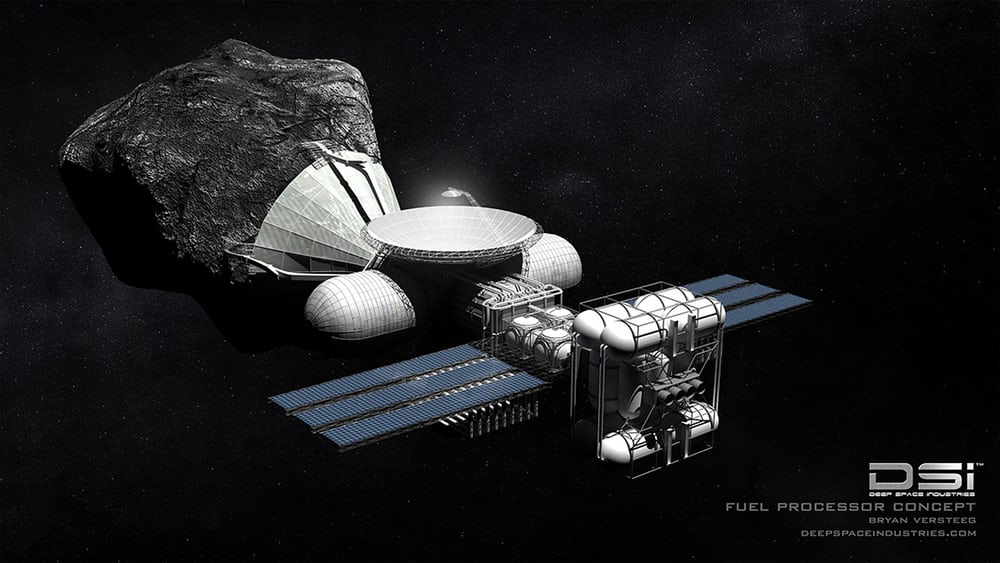
\includegraphics[height=8.5cm]{figures/asteroid-mining-feature-8.jpg}%
	        \caption*{Asteroid Mining}%
        \end{subfigure}~\hfill 
        \begin{subfigure}[b]{0.4\columnwidth}%
            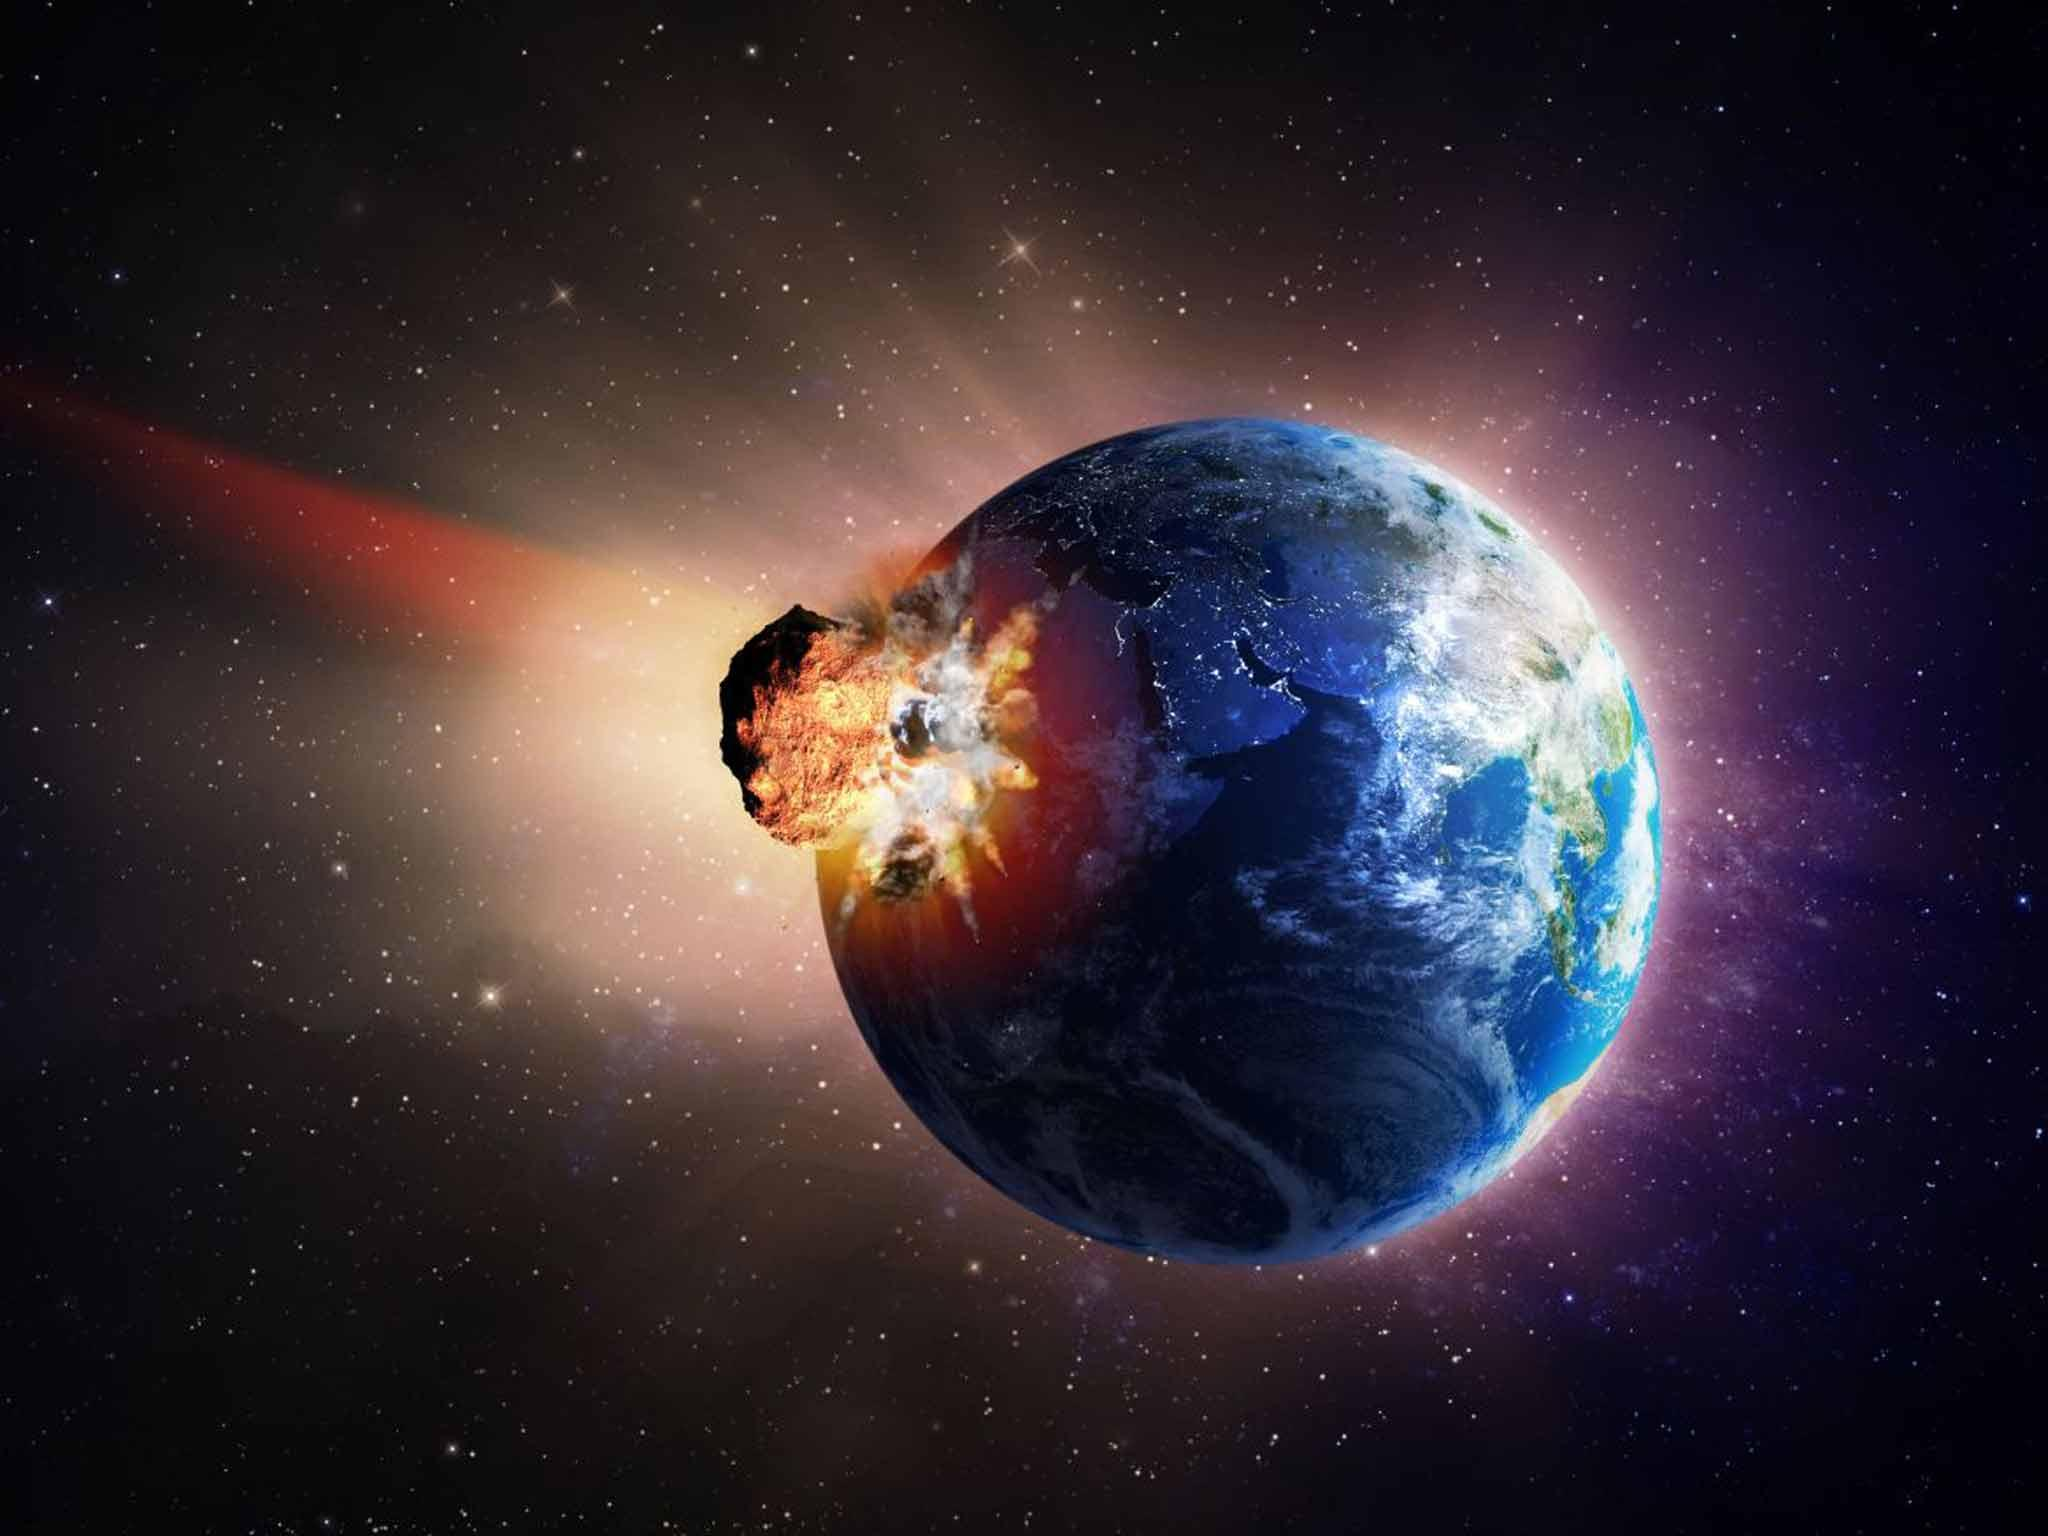
\includegraphics[height=8.5cm]{figures/asteroid-alamy.jpg}%
            \caption*{Asteroid Impact}%
        \end{subfigure}%
        \hfill%
	\end{figure}
\end{block} % end of background block

\begin{block}{Motivation}
	\begin{itemize}
		\item \Emph{You can emphasize stuff} 
		\item The blocks are all top aligned. 
		\item You can change this in the command \texttt{column}
	\end{itemize}
\end{block} 

\begin{block}{Background}
	\begin{itemize}
		\item \Emph{You can emphasize stuff} 
		\item The blocks are all top aligned. 
		\item You can change this in the command \texttt{column}
	\end{itemize}
\end{block} 

\end{column}  % first column end

%-----------------------------------------------------------------------------------------
% SECOND (WIDE MIDDLE) COLUMN
%---------------------------------------------------------------------------------------
\begin{column}{\twocolwidth} % second column start

\begin{block}{Optimal Control - Reachability} % structure block
	\begin{minipage}{0.5\columnwidth} % left half of this block
	\begin{itemize}
		\item This block is split into two using \texttt{minipage}
			\begin{align*}
				\mathsf{S}^2 = \left\{q \in \mathsf{R}^3 \,  \vert \, \| q \| = 1 \right\}
			\end{align*}
		\item Lots of fancy equations
	\end{itemize}
	\end{minipage}% end of left half of block
	\begin{minipage}{0.5\columnwidth}% right half of block
		\begin{itemize}
			\item Now we're into the right half of the block
				\begin{align*}
					\Psi(R) = A(R) B(R) 
				\end{align*}
			\item More equations few will understand or care about
		\end{itemize}
	\end{minipage}%end of right half of block
	
	\begin{itemize}
		\item All of this will span the width of the entire column.
		\item Since it is after the \texttt{minipage} environment
	\end{itemize}
\end{block} % end of structure block

\begin{block}{Numerical Simulation} % optimal control block
	\begin{itemize}
		\item \Emph{Spans the entire column width} 
		\begin{align*}
			\text{Initial: } R_0 =  \exp(\ang{225} \times \frac{\pi}{180} \hat{e}_3) \quad \text{Final: } R_d = I \quad \text{Disturbance: } \Delta = \begin{bmatrix} 0.2 & 0.2 & 0.2 \end{bmatrix}^T
		\end{align*}
		\item SCIENCE!
	\end{itemize}
\end{block} % end of optimal control block
\end{column}


%-----------------------------------------------------------------------------------------
% THIRD (RIGHT) COLUMN
%---------------------------------------------------------------------------------------
\begin{column}{\onecolwidth} % third column start

\begin{block}{Novel benefits} % results block
	\begin{itemize}
		\item Make sure to talk about how awesome your research is
	\end{itemize}
\end{block} % end of results block

\begin{block}{Conclusions} % conclusion
	\begin{itemize}
		\item Remind them about everything you already told them
		\item They should be quite amazed by this point
	\end{itemize}
\end{block} % conclusion
\end{column}  % third column end

\end{columns} % end of all columns in poster
\end{frame} % end of enclosing frame
\end{document}